\documentclass[10pt]{beamer}

\usetheme{metropolis}
\usepackage{appendixnumberbeamer}

\usepackage{booktabs}
\usepackage[scale=2]{ccicons}
\usepackage{graphicx}
\usepackage{hyperref}
\usepackage{circuitikz}
\usepackage{pdflscape}
\usepackage{smartdiagram}

\usepackage{color}
\usepackage{listings}

\lstset{
	basicstyle=\footnotesize\ttfamily,
    keepspaces=true,
    showstringspaces=false,
    language=PHP,
    commentstyle=\ttfamily,
}

\usepackage[OT4]{polski}
\usepackage[utf8]{inputenc}

\usepackage{pgfplots}
\usepgfplotslibrary{dateplot}

\usepackage{xspace}
\newcommand{\themename}{\textbf{\textsc{metropolis}}\xspace}

\setbeamertemplate{frame footer}{}
\setbeamertemplate{frame numbering}{}

\usetikzlibrary{shapes,arrows}

\tikzstyle{decision} = [diamond, draw, fill=blue!20, 
    text width=4.5em, text badly centered, node distance=3cm, inner sep=0pt]
\tikzstyle{block} = [rectangle, draw, fill=blue!20, 
    text width=5em, text centered, rounded corners, minimum height=4em]
\tikzstyle{line} = [draw, -latex']
\tikzstyle{cloud} = [draw, ellipse,fill=red!20, node distance=3cm,
    minimum height=2em]


\title{Architektura sterowana zdarzeniami}

\subtitle{Zaawansowane metody programowania}
\author{mgr inż. Krzysztof Rewak}
\date{\today}
\institute{Wydział Nauk Technicznych i Ekonomicznych \\ Państwowa Wyższa Szkoła Zawodowa im. Witelona w Legnicy}

\begin{document}

\maketitle

\begin{frame}{Plan prezentacji}
  \setbeamertemplate{section in toc}[sections numbered]
  \tableofcontents[hideallsubsections]
\end{frame}


\section{Obserwatorzy}

\begin{frame}{Jesteś obserwowany}
	Zanim przejdziemy do omawiania aplikacji sterowanych zdarzeniami, chciałem krótko przypomnieć o wzorcu projektowym \textbf{obserwator} (ang. \emph{observer}).
\end{frame}

\begin{frame}{UML}
	\begin{figure}[t]
		\centering
		\includegraphics[width=\linewidth]{observer.png}
		\caption{Diagram UML obserwatora}
	\end{figure}
\end{frame}

\begin{frame}[fragile]{Wzorzec Obserwator}
\begin{lstlisting}
public class User implements Observer {
 
    @Override
    public void create(Observable observable) {
        observable.createEmptyProfile();
    }
    
}
\end{lstlisting}
\end{frame}

\begin{frame}{Obserwatorzy}
	Współczesne frameworki zazwyczaj umożliwają obserwowanie poprzez podpięcie się do kilku \emph{zdarzeń} towarzyszących modelom.
\end{frame}

\begin{frame}{Obserwatorzy}
	Przykładowo mogą to być:

	\texttt{retrieved, creating, created, updating, updated, saving, saved, deleting, deleted, restoring, restored}.
\end{frame}

\begin{frame}{Obserwatorzy}
	Korzystanie z obserwatorów to pierwszy krok do korzystania z architektury sterowanej zdarzeniami.
\end{frame}

\section{Zdarzenia}

\begin{frame}[fragile]{MVC}
	\hspace*{1.25cm}%
	\begin{tikzpicture}[node distance=4cm, minimum size=2cm, auto]
	
		\node [circle, fill=orange,inner sep=3pt] (user) {użytkownik};
		
		\node [block, above right of=user] (controller) {kontroler};
		\node [block, above left of=user] (view) {widok};
		\node [block, above left of=controller] (model) {model};
		
	
		\path [line] (user) -- node[label={[shift={(2,-3.5)}]wywołuje}] {} (controller);
		\path [line] (controller) -- node[label={[shift={(2,-0.5)}]żąda zmian}] {} (model);
		\path [line] (model) -- node[label={[shift={(-2,-0.5)}]uaktualnia}]  {} (view);
		\path [line] (view) -- node[label={[shift={(-2,-3.5)}]wyświetla}] {} (user);
	\end{tikzpicture}
\end{frame}

\begin{frame}[fragile]{MVC... MRMSE?}
	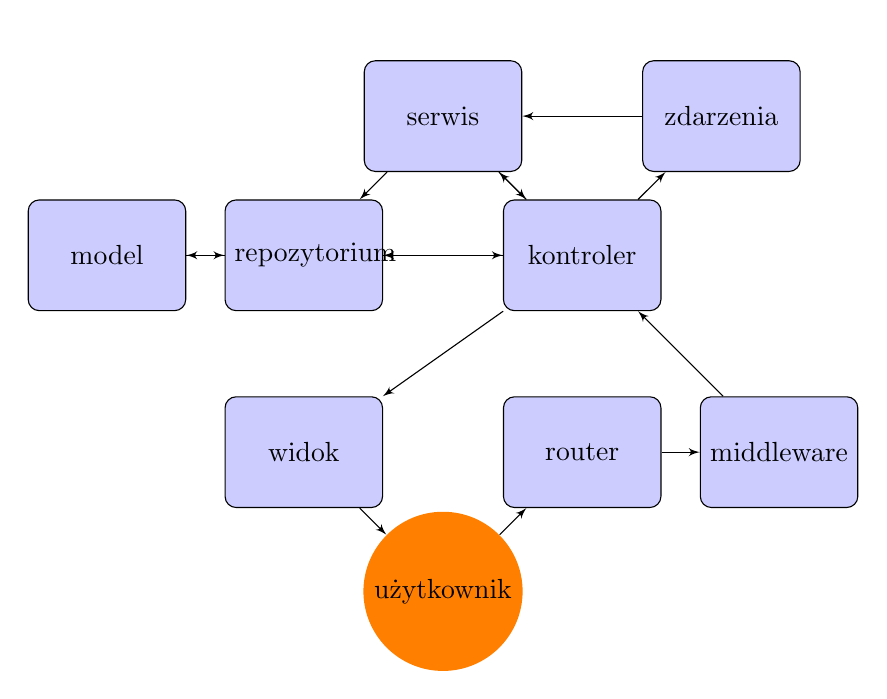
\begin{tikzpicture}[node distance=2.5cm, minimum size=2cm, auto]
	
		\node [circle, fill=orange,inner sep=3pt] (user) {użytkownik};
		
		\node [block, above right of=user] (router) {router};
		\node [block, above left of=user] (view) {widok};
		\node [block, right of=router] (middleware) {middleware};
		
		\node [block, above of=router] (controller) {kontroler};
		\node [block, above of=view] (repo) {repozytorium};
		\node [block, left of=repo] (model) {model};
		
		\node [block, above left of=controller] (service) {serwis};
		\node [block, above right of=controller] (event) {zdarzenia};
		
		\path [line] (user) -- node {} (router);
		\path [line] (router) -- node {} (middleware);
		\path [line] (middleware) -- node {} (controller);
		\path [line] (controller) -- node {} (service);
		\path [line] (controller) -- node {} (event);
		\path [line] (event) -- node {} (service);
		\path [line] (service) -- node {} (repo);
		\path [line] (controller) -- node {} (repo);
		\path [line] (repo) -- node {} (model);
		\path [line] (controller) -- node {} (view);
		\path [line] (view) -- node {} (user);
		
		\path [line] (service) -- node {} (controller);
		\path [line] (repo) -- node {} (controller);
		\path [line] (model) -- node {} (repo);
	\end{tikzpicture}
\end{frame}

\begin{frame}{Zdarzenia?}
	Proste aplikacje webowe często zachowują się algorytmicznie lub strukturalnie: pobierz zapytanie, zwaliduj dane, uruchom serwis, zapisz coś w bazie danych, wygeneruj powiadomienie, zwróć wynik. 
	
	Wiele rzeczy robimy w kontrolerach lub wydzielonych serwisach właśnie w taki sposób. 
\end{frame}

\begin{frame}[fragile]{Co tu nie gra?}
\begin{lstlisting}
def signup(request):
  form = SignupForm(request.POST)
  user = form.save(commit=False)
  user.save()

  mail_subject = 'Activate your blog account.'
  message = render_to_string('activate_user.html', {
    'user': user,
    'token': account_activation_token.make_token(user),
  })

  to_email = form.cleaned_data.get('email')
  email = EmailMessage(mail_subject, message, to=[to_email])
  email.send()
  
  return HttpResponse('Confirm your email address.')
\end{lstlisting}
\end{frame}

\begin{frame}{Co tam nie gra?}
	Przede wszystkim rzuca się oczy możliwość stworzenia serwisu rejestrującego użytkownika i wysyłającego email...
	
	... albo dwóch osobnych serwisów to robiących i wywołanych w kontrolerze...
	
	... albo wywołaniu jednego w drugim?
\end{frame}

\begin{frame}{Zdarzenia!}
	A gdyby zamiast tworzyć (lub przekazywać przez wstrzyknięcie zależności) nową instację serwisu można byłoby krzyknąć do aplikacji: \emph{ej, weź wyślij mejla}?
\end{frame}

\begin{frame}[fragile]{Lepiej?}
\begin{lstlisting}
def signup(request):
  form = SignupForm(request.POST)
  user = form.save(commit=False)
  user.save()

  send_activation_email.send(self, user)
  
  return HttpResponse('Confirm your email address.')
\end{lstlisting}
\end{frame}

\begin{frame}{Słuchanie zdarzeń}
	Oczywiście ktoś musi słuchać naszego krzyczenia. Każdy framework definiuje to w nieco inny sposób, ale idea zazwyczaj jest taka sama: potrzebujemy \emph{listenera}, który przetworzy nasze zdarzenia.
\end{frame}

\begin{frame}[fragile]{Słuchanie zdarzeń}
\begin{lstlisting}
class OrderShipped {
  public $order;
  
  public function __construct(Order $order) {
      $this->order = $order;
  }
}

class SendShipmentNotification {

    public function handle(OrderShipped $event) {
        $event->(...);
    }

}

// (...)

event(new OrderShipped($order));
\end{lstlisting}
\end{frame}

\begin{frame}{Czego słuchać?}
	Wszystkiego, czego odpowiedzi tak naprawdę nie potrzebujemy.
	
	Zastanówmy się jak wiele takich akcji realizowanych jest w naszych projektach? Wszystko, co związane z wysyłaniem mejli, zapisywaniem plików, bardzo często ze zmianami w bazie danych.
\end{frame}

\section{Kolejkowanie zdarzeń}

\begin{frame}{Kto pierwszy, ten lepszy?}
	Skoro wynik niektórych operacji jest dla nas czasami nieistotny i możemy realizację takiego zadania przerzucić na zdarzenie/słuchacza to może warto byłoby zastanowić się czy te zdarzenia muszą sie wykonać synchronicznie?
\end{frame}

\begin{frame}{Kto pierwszy, ten lepszy?}
	Przyjmijmy, że wysyłanie mejla to skomplikowana sprawa. Trzeba się połączyć z serwerem poczty, wyciągnąć z bazy danych użytkownika, przerenderować wiadomość i oczywiście ją wysłać. Trwa to stosunkowo długo i czy faktycznie użytkownik musi czekać na koniec zadania żeby otrzymać powiadomienie \emph{Odbierz mejla i aktywuj konto}?
\end{frame}

\begin{frame}{Kolejkowanie zdarzeń}
	\begin{figure}[t]
		\centering
		\includegraphics[width=\linewidth]{queue.jpg}
		\caption{Idea kolejkowania zdarzeń}
	\end{figure}
\end{frame}

\begin{frame}{Kolejkowanie zdarzeń}
	Można utworzyć w dowolny sposób kolejkę zdarzeń do wykonania i następnie za jej pomocą zarządzać ich wykonywaniem. 
\end{frame}

\begin{frame}{Kolejkowanie zdarzeń}
	Korzystając z brokera wiadomości (RabbitMQ, Celery, Redis) można stworzyć kolejkę wewnątrz serwisu lub łącząc ze sobą (mikro)serwisy.
\end{frame}

\section{EDA}

\begin{frame}{\emph{Event-driven architecture}}
	Naturalnym rozwinięciem idei zdarzeń będzie architektura sterowana zdarzeniami, czyli \emph{Event-driven architecture}, EDA.
\end{frame}

\begin{frame}{\emph{Event-driven architecture}}
	Najpierw definicje: \textbf{zdarzenie} powinno być interpretowane wówczas jako zmianę w stanie danego systemu.
\end{frame}

\begin{frame}{Maszyna stanu}
	\begin{figure}[t]
		\centering
		\includegraphics[width=.75\linewidth]{state.png}
	\end{figure}
\end{frame}

\begin{frame}{\emph{Event-driven architecture}}
	Przy EDA zdarzenia nie są klasami samymi w sobie, a bardziej ustandaryzowanymi komunikatami, które przesyłane są do konsumentów. Taki \emph{event} najczęściej zawiera w sobie nazwę, timestamp, flagę typu zdarzenia oraz dodatkowe dane, które będą potrzebne przy przetwarzaniu zdarzenia.
\end{frame}

\begin{frame}{\emph{Event-driven architecture}}
	A więc: zmiena się stan użytkownika; przykładowo flaga \texttt{active} zmieniła swoją wartość z \texttt{true} na \texttt{false}. System powinien wyłapać taką zmianę i rozpropagować wiadomość informującą o tym zdarzeniu.
	
	Każdy mikroserwis wchodzący w skład systemu odnotuje tę informację i zrobi to, co uzna za stosowne. 
\end{frame}

\begin{frame}{\emph{Event-driven architecture}}
	\begin{figure}[t]
		\centering
		\includegraphics[width=.75\linewidth]{eda.png}
	\end{figure}
\end{frame}

\begin{frame}{\emph{Event-driven architecture}}
	EDA może być potężnym narzędziem. Jest również coraz bardziej popularniejszym rozwiązaniem w projektach zarówno komercyjnych, jak i opensourcowych, więc warto się z nim zapoznać.
\end{frame}

\section{Podsumowanie}

\begin{frame}{Bibliografia i ciekawe źródła}
  
	\begin{thebibliography}{9}
		
		\bibitem{observer}
		\url{https://en.wikipedia.org/wiki/Observer_pattern}
		
		\bibitem{laravel}
		\url{https://laravel.com/docs/5.6/eloquent\#observers}
		
		\bibitem{queue}
		\url{https://docs.microsoft.com/en-us/dotnet/standard/microservices-architecture/multi-container-microservice-net-applications/integration-event-based-microservice-communications}
		
		\bibitem{eda}
		\url{https://en.wikipedia.org/wiki/Event-driven_architecture}
		
		\bibitem{state}
		\url{https://brilliant.org/wiki/finite-state-machines/}
		
		\bibitem{eda}
		\url{https://wso2.com/blogs/thesource/2016/05/how-you-can-increase-agility-and-expandability-with-event-driven-architecture-eda/}
	
	\end{thebibliography}

\end{frame}

\appendix

\begin{frame}[standout]
	Pytania?
\end{frame}

\begin{frame}{}

	Kod prezentacji dostępny jest w repozytorium git pod adresem \texttt{https://bitbucket.org/krewak/pwsz-zmp} \\ \ \\

	\begin{figure}
		\centering
		\href{https://bitbucket.org/krewak/pwsz-ppsi}{
			\includegraphics[width=.15\textwidth]{../_template/bitbucket.png}
		}
	\end{figure}
	
	Wszystkie informacje dot. kursu dostępne są pod adresem \texttt{http://pwsz.rewak.pl/kursy/10} \\ \ \\

	\begin{figure}
		\centering
		\href{http://pwsz.rewak.pl/kursy/3}{
			\includegraphics[width=.15\textwidth]{../_template/rewak.png}
		}
	\end{figure}

\end{frame}

\end{document}
